\documentclass[10pt]{book}
\usepackage{graphicx}
\usepackage{subfig} % make it possible to include more than one captioned figure/table in a single float
\usepackage[utf8]{inputenc}
\usepackage{amsmath}
\setlength{\oddsidemargin}{15.5pt} 
\setlength{\evensidemargin}{15.5pt}
\pretolerance=2000
\tolerance=3000
\renewcommand{\figurename}{Figura}
\renewcommand{\chaptername}{Cap\'{i}tulo}
\renewcommand{\contentsname}{\'{I}ndice}
\renewcommand{\tablename}{Tabla}
\renewcommand{\bibname}{Bibliograf\'{i}a}
\renewcommand{\appendixname}{Ap\'endices}


\title{Análisis de diagrama HR}
\date{}
\begin{document}
\section*{Introduccion}



  El diagrama de Hertzsprung-Russell(HR) muestra el resultado de numerosas observaciones sobre la relación existente entre la magnitud absoluta de una estrella(luminosidad) y tipo espectral(temperatura efectiva).
El diagrama donde se muestra Mi como función del color (Mv - Mi) con axis Y invertido(ColorMagnitudeDiagram) es equivalente al diagrama donde se representa la luminosidad frente a la temperatura efectiva con axis X invertido(HR original). Las curvas de las isocronas en los 2 diagramas son similares (testiso.py). 
Las galaxias evoluan de 2 formas: dinámica por interacciones con otros sistemas y a través del proceso de formación y evolución de las estrellas. Este proceso determina el proceso de enriquecimiento químico del medio en donde se van a formar futuras estrellas así que la historia de formación estelar(StarFormationHistory) es fundamental para entender la evolución de una galaxia. 
El diagrama CMD es la mejor herramienta para estudiar la SFH de
una galaxia porque muestra estrellas formadas en diferentes momentos de su vida.

Las estrellas, independiente de su masa inicial pasan la mayor parte de su vida en la secuencia principal quemando hidrógeno en el núcleo. Después empiezan a quemar H en una capa y de este punto la evolución será diferente dependiendo de su masa:
\begin{itemize}
\item En las estrellas de baja masa el núcleo de He no tiene la densidad y temperatura necesaria para empezar la combustión, el núcleo se contracta, aparece la degeneración de los electrones. 
Las estrellas suben por la rama RedGiantBranch mientras H se está quemando en la capa y el He se acumula en el núcleo hasta que este llegue a una masa 0.45-0.55 Msol y una temperatura alta  que He empieza a quemarse de forma explosiva(por la degeneración: flash de He) y la degeneración desaparece. La estrella acaba la fase RGB y empieza por la Horizontal Branch cuando H y He se queman en el núcleo y la capa. La luminosidad máxima en la rama RGB y la luminosidad de las estrellas en HB son casi constantes porque el núcleo en el momento del flash de He  tiene casi la misma masa.
\item En las estrellas de masa intermedia y masivas el He empieza a quemarse en un núcleo no degenerado. Al principio de esta fase la estrella está cerca de la línea Hayashi, pero luego cuando la energía producida en el núcleo por el He es igual a la energía producida por el H en la capa la capa exterior de la estrella se contracta y deviene radiativa, la tempertaura crece y la estrella se encuentra en la zona Blue Loop. La luminosidad en esta fase crece con la masa de la estrella.
\end{itemize}
Después la combustión de He un núcleo de C-O está formado, H y He quemandose en capas

\begin{itemize}
\item En las estrellas de masa pequeña e intermedia la masa del núcleo C-O es constante no suficiente para que el núcleo C-O empieza a quemarse y aparece de nuevo la degeneración eléctronica en el núcleo. 
El núcleo se contrae, la capa de He se expande y la capa exterior de H se contrae(efecto espejo: 2 espejos). La temperatura en la capa de H baja y la combustión del H en la capa se para y ahora las 2 capas de He y H se expanden como reacción a la contracción del núcleo(efecto espejo)
Es una fase larga cuando la luminosidad de la estrella es determinada solo por la energía de la combustión de He hasta, el He se agota en la parte mas cerca del núcleo y la capa de He se acerca cada vez mas a la capa de H (la fase Early-AGB). 
Cuando la capa de He está muy cerca a la capa de H esta se enciende de nuevo y aparecen flash de He: la tempertaura oscila en la capa de He(los pulsos termicos de la fase AGB: TP-AGP). En esta fase la estrella pierde masa y después se transforma en una enana blanca
\item En las estrellas masivas la masa del núcleo C-O crece con la masa de la estrella y este empieza a quemarse(no aparece la degenaración ) y después empieza la nucleosintesis de elementos con masa atómica mas grande hasta llegar al hierro cada vez a temperaturas mas grandes. La vida de la estrella en esta fase es muy corta(hasta la explosión como una supernova).
\end{itemize}




\section*{Datos de entrada}
\subsection*{Tablas de isocronas}

Las tablas de las isocronas están representados por ficheros distintos para cada metalicidad (usamos "isocz0004.dat" , "isocz001.dat",  "isocz004.dat" , "isocz008.dat", "isocz019.dat", "isocz030.dat") con varias columnas de cuales nos interesan: 1 log(edad), 2 masa inicial, 10 Mv magnitud absoluta en el filtro pasa banda V, 12 Mi magnitud absoluta en el filtro pasa banda I.
Los ficheros están generados por un modelo de evolución estelar que muestra la evolución en el tiempo dependiendo de la masa inicial y composición química de las demás  propiedades de la estrella(Luminosidad, magnitudes en varios filtros, temperatura efectiva, gravedad,...) que se pueden ver como funciones discretas de los siguientes parametros:

\begin{itemize}
	\item la edad de la estrella\\
	El tiempo inicial(0) es considerado el momento cuando la estrella entra en secuencia principal ZAMS
	Se calcula para edades e con $7.8 \le log(e) \le 10.25$ step 0.05

	\item masa inicial\\
	Se calcula para masas iniciales $\ge$ 0.15 y hasta la masa maxima que puede existir con esta edad MIniMax(edad). Los valores son dados en unidades de masa solar
	En las estrellas de masa baja (aprox 0.6)  la evolución se para en la fase de pulsaciones termicas AGB(el proceso salta la fase del flash de He que requiere mucho tiempo del CPU). En las estrellas de masa intermedia la evolucion para en el comienzo de  la fase TP-AGP y en las estrellas masivas cuando C empieza a quemarse.

	\item metalicidad. En realidad los modelos de evolucion toman como parámetro la composisión química(expresada por cantidades relativas a 1: X para H, Y para He , Z(metalicidad) para suma de las cantidades de los demás elementos). En este caso hay una relación fija entre Y y Z así que el único parametro real es Z
\end{itemize}



\subsection*{Diagrama Magnitud-Color a analizar}

(dhr7.dat) fue creado con el programa iac-star que genera un diagrama color magnitud sintetico \\

\textbf{Parametros de entrada}
\begin{description}
\item InitialMassFunction = f([m1,m2]) - numero de estrellas que se forman con masa entre m1 y m2. 
	\begin{description}
	\item Se intoducen los valores $ n, m_1, .. m_n, x_1, x_2, .. x_{n-1}$ 
 	\item $IMF([m_i,m_{i+1}]) =  K * m_i  ^ {-x_i} \forall i \in [1..n-1]$, K calculado internamente
\end{description}
\item StarFormationRate = f(t) - numero de estrellas que se forman en un momento dado. Aquí se define también la EdadTotal
	\begin{description}
	\item introducir los valores $n, t_1, t_n, ..SFR(t_1), SFR(t_n)$, $t_n$ representa la EdadTotal
	\item introducir 1, EdadTotal , $\beta$	estos ultimos 2 son parametrso para la funcion predefinida $SFR(t) = e^{t/(-\beta)}$
	\end{description}
\item ChemicalEnrichmentLaw = f(t) - la metalicidad en un momento dado. 
Se puede definir de forma opcional aparte de la funcion principal(lower or unique: CEL1(t))  otra función(upper: CEL2(t)) para tener dispersión en la metalicidad: no todas las estrellas que se forman en un momento tienen que tener la misma metalicidad: la metalicidad sera un valor arbitrario entre CEL1(t) y CEL2(t)

 Las definiciones se pueden hacer de 2 formas: 
	\begin{itemize}
		\item introducir los valores $n, t_1, t_n, ..CEL(t_1), CEL(t_n)$
		\item introducir parametros($Z_i$, $Z_f$, final gas fraction, infall, outflow) para unas funciones predefinidas (que son funciones crecientes en el tiempo?)
	\end{itemize}
\item edad total
\item tablas de isocronas que definen Mv(edad,metalicidad, masaInicial) y Mi(edad, metalicidad, masaInicial) - funciones discretas 
\end{description}
\emph{Nota}: No he tenido en cuenta la formación de estrellas binarias y la perdida de masa porque no se pueden relacionar directamente con las tablas de las isocronas


\textbf{Descripción del algoritmo para generar dhr7.dat}
\begin{description}
\item forall t in 0..EdadTotal
\begin{description}
	\item se calcula  el numero de estrellas que se forman en este momento N = SFR(t)
	\item forall k from 1 to N
		\begin{description}
			\item en funcion de la IMF introducida se determina la masaInicial de las estrella 
			\item edad = EdadTotal-t, 
			\item metalicidad = CEL(t)
			\item se calcula Mv(edad,metalicidad,mi) y Mi(edad, metalicidad,masaInicial) y se introducen en el fichero los valores para el color = Mv - Mi y Mi \\
			
	
		\end{description}
			
\end{description}
\item CEL(si se introduce), SFR; Mv y Mi de las tablas de isocronas son funciones discretas, los valores para cualquier entrada se calcula por interpolacion 
\end{description}

\section*{Metodo de análisis}

De las tablas de isocronas se pueden definir la isocronas como  funciones de la edad y metalicidad  que tiene como valor un conjunto de puntos en el diagrama  magnitud-color(calculados para todas las estrelas con todss masas iniciales posibles con esta edad y metalicidad) Como en práctica solo se calcula para valores discretos de la masa inicial(determinados por una distribución de masas IMF elegida) podemos unir los puntos y aproximar la posicion de cualquier estrella(cualquier masa inicial: no sabemos si IMF es siempre la misma) con la respectiva edad y metalicidad  en esta linea.\\

\textbf{Interpretación gráfica de las isocronas}
\begin{itemize}
\item Relación con la masa inicial: Las estrellas con masa menor están en la parte abajo de las isocronas(tienen una evolución más lenta) (testisomi.py)
\item Relación con la metalicidad: La isocrona para estrellas con mas metalicidad está siempre más a la derecha (testisoz.py)
y por abajo.
Mas metalicidad implica menor temperatura y menor luminosidad(la metalicidad es una fuente de opacidad y  una estrella tendrá un radio menor que otra con mas metalicidad y la misma masa. Además en las ultimas etapas las estrellas con mas metalicidad pierden mas masa)
\par Observando la decomposición en isocronas de los diagramas de los cúmulos globulares(donde se supone que todas las estrellas tienen metalicidad parecida), las isocronas para edad mayor están más a a la derecha y abajo (la distancia entre ellas sobre todo se observa en la zona turnoff de la secuencia principal)

\begin{figure}[!h]
 \centering
 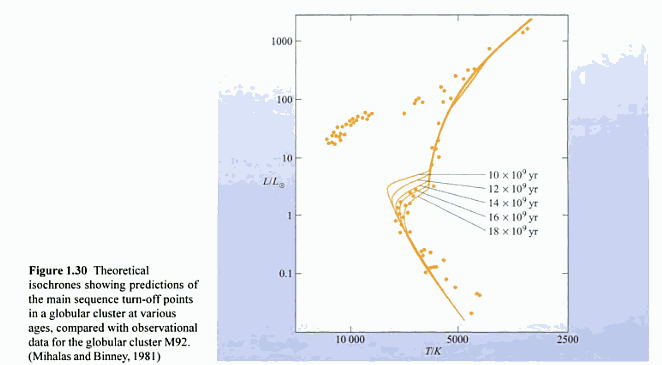
\includegraphics[scale=0.7]{gciso.png}
 \caption{\emph{Estimacion de la edad de un cumulo globular}}
 \label{Fig: 2}
\end{figure}
\end{itemize}

\textbf{Procedimiento}
\begin{itemize}
 \item Hay que descomponer el diagrama CMD en las isocronas que lo componen: cada una representa un episodio de formación estelar(determinar la funcion SFR y CEL)
\item Desarrollo de una aplicación grafica en python usando wx y matplotlib 
	\item Representamos las isocronas por lineas  por la razón explicada antes. La IMF usada puede ser diferente. Tambien pueden haber en la galaxia (de nuesteo diagrama) estrellas de edad y metalicidad que no se encuentran en las tablas de isocronas(recoradar que en iac-star estos valores se calculan por interpolación). Ademas usando tablas de isocronas diferentes la posición en el diagrama no va a coincidir exactamente con el punto de la isocrona incluso para los mismos valores de la masa inicial, edad y metalicidad
\item En nuestro diagrama parece haber elegido solo masas iniciales a partir de un cierto rango(0.7) (se puede especificar en el programa) porque el diagrama parece cortado por abajo(determinar IMF)
\item Si se ha introducido la segunda función CEL(y solo en este caso) podemos encontrar en el diagrama varias isocronas para la misma edad, pero para metalicidades distintas
\item Hacemos un analisis empirico cualitativo del diagrama(no hay estrellas en la secuencia principal , pero RGB esta bien definida igual que la zona de los HB y AGB parece bien poblada lo que significa que no hay formacion estelar reciente y que la IMF favorece la formación de estrellas de baja masa: además veremos que las estrellas en la rama HB tendrán la edad más grande lo que significa que las estrellas en esta zona tendrán una masa mucho menor que las estrellas de la zona AGB con edad más pequeña: las fase AGB es después de la fase HB en la evolución de una estrella) y miramos la representación de todas las isocronas para cada metalicidad(testisomi.py, testisomiall.py) 
\item Se ejecuta el programa:
\begin{verbatim}
	python wxhr.py -l listiso -i dhr7.dat
\end{verbatim}
donde
\begin{description}
	\item listiso es un fichero con todas las isocronas que se cargan al principio
	\item dhr7.dat el fichero del diagrama a analizar	
\end{description}

\item En el programa se pueden cargar tablas de isocronas (para una metalicidad) elegir las isocronas que se representan para cada una(tambien mostrarlas y ocularlas por grupo), definir la masa inicial minima para cual se representan las isocronas, seleccionar las isocronas en el grafico. Hay una demonstración(grabación de pantalla): video.mkv y leer el readme
\item La edad total es 17.78 (consideramos la edad maxima presente en la tabla de las isocronas log(edad) = 10.25 que es presente como isocrona en el diagrama)
\item Consideramos formación continua en el intervalo[$t_1$, $t_2$]  si existen isocronas para todas las edades en el intervalo log(e) in [$edad_1$, $edad_2$,  (step=0.05)], $t_1=EdadTotal - 10^{edad_2}, t_2=EdadTotal - 10^{edad_1}$. De forma similar definimos CEL1 = z1 y CEL2 = z2 en el intervalo [$t_1, t_2$] si z1=$\displaystyle \min_{i \in isochrones(edad)} metalicity(i)$ y z2=$\displaystyle \max_{i \in isocrones(edad)} metalicity(i)$ para todas las edades  en el intervalo log(edad) in [$edad_1$, $edad_2$,  (step=0.05)]. Mirar Help,About en el menu del programa
\item Comprobamos los resultados en iac-star con los siguentes parametros que representan mas o menos la salida del programa de Fig1
He considerado SFR = 1 en los intervalos donde hay formación continua: 2 episodios de formación estelar entre tiempo [0..3.66]Gy y [7.78..15.28]Gy - no hay ninguna isocrona para log(age) in \{10.05, 10.1\}, tiempo = EdadTotal - edad; la metalicidad es entre 0.0004 y 0.008, he modificado un poco las funciones  CEL1 y CEL2 para que sean crecientes(en general la metalicidad crece en el tiempo porque al final de su vida las estrellas enriquecen el medio interestelar con los metales producidos durante ella) y tengo en cuenta que la IMF favorece las estrellas con masa inicial baja

\begin{description}

\item SFR = 8, 0, 3.66, 3.67, 7.77, 7.78, 15.27 , 15.28,17.78, 1,1,0,0,1,1,0,0
\item CEL1=6, 0, 3.66, 10.7, 12.77, 14.23, 17.78,  0.0004, 0.001, 0.004, 0.004, 0.008, 0.008
\item CEL2= 6, 0, 3.66, 10.7, 12.77, 14.23, 17.78,  0.0004, 0.004, 0.004, 0.008, 0.008, 0.008
\item IMF=3, 0.7, 1, 120., -1.3, -2.3  
\end{description}


\item Comparamos los resultados de iac-star y nuestro diagrama dhr7.dat y vemos que son parecidos (Figura2) (Hay que tener en cuenta que iac-star por la dispersion de masa inicial y metalicidad no genera siempre el mismo diagrama aunque ejecutado con los mismos parametros) 
\begin{verbatim}
	python testiacstar.py cmd_31607 dhr7.dat
\end{verbatim}


\begin{figure}[!h]
 \centering
 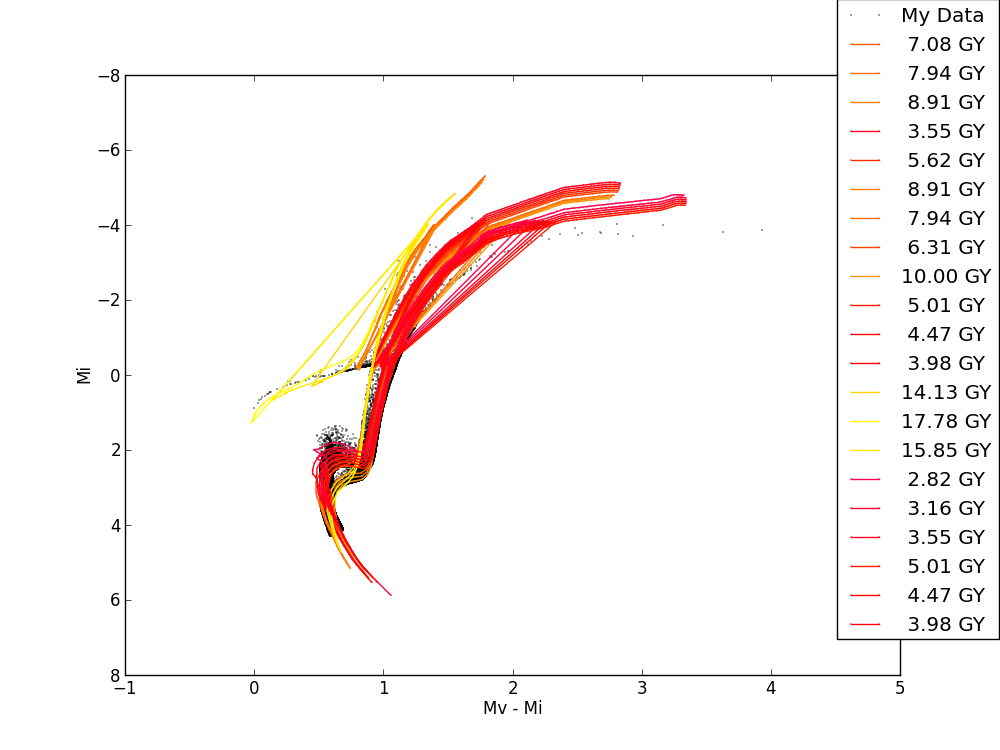
\includegraphics[scale=0.7]{alllines.png}
 \caption{\emph{Isocronas}}
 \label{Fig: 1}
\end{figure}

\begin{figure}[!h]
 \centering
 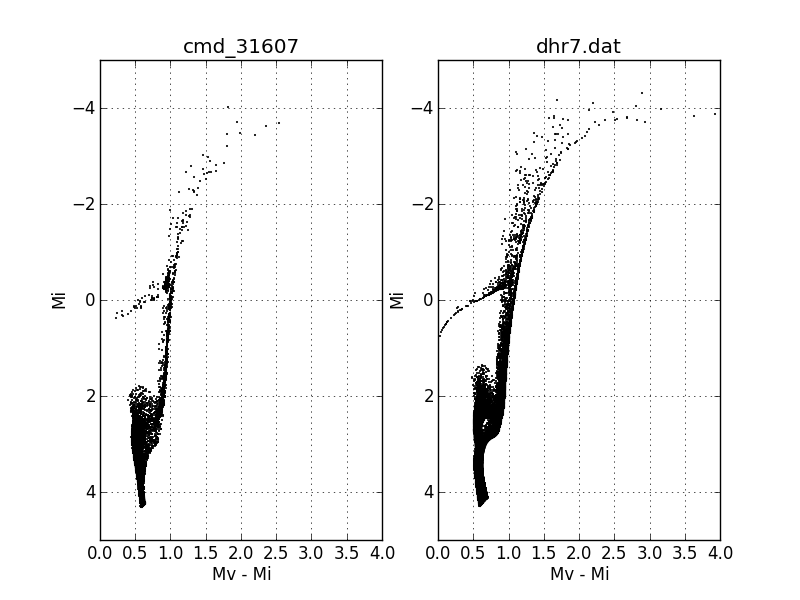
\includegraphics[scale=0.7]{cmd_31607.png}
 \caption{\emph{Comparación salida iac-star y  dhr7.dat}}
 \label{Fig: 2}
\end{figure}
\end{itemize}






\section*{Resultados}
Todo se encuenta en un repositorio en github(incluso paper.pdf y aparicio.pdf que sirvieron como documentación para hacer la práctica) en la dirección: https://github.com/beevageeva/astro/tree/master/HR/

Se puede bajar completo con git:
\begin{verbatim}
git clone https://github.com/beevageeva/astro/tree/master/HR/  
\end{verbatim}
o mirar el contenido con el navegador








 





\end{document}

